
\documentclass[11pt, a4paper]{book}
\input{package.tex}
\pgfplotsset{compat=1.17}
\begin{document}
\chapter{Représentation numérique de l’information}


\section{Introduction}

Aujourd’hui, nous utilisons des ordinateurs, des téléphones mobiles, des tablettes pour écrire, regarder des vidéos, écouter de la musique ou jouer à des jeux. Mais comment une machine peut-elle comprendre autant de choses différentes ?

Lorsque nous utilisons un logiciel, chacune de nos actions, réalisée par exemple avec la souris ou le clavier, est traduite en langage informatique avant d'être exécutée par l'ordinateur. 

\begin{quotation}
\itshape “Transmettre des informations sous forme numérique suppose entre autres d'optimiser la taille des messages transmis pour éviter de surcharger les canaux de transmission, d'être capable de rectifier des erreurs apparues en cours de transmission, de crypter les contenus et d'authentifier les émetteurs et les destinataires…”
\raggedleft
(Dunod, 2006)
\end{quotation}

Les images, les sons, les textes et les vidéos sont autant d'informations qu'un ordinateur peut traiter. Un ordinateur est constitué de circuits électroniques qui manipulent des signaux électriques. À l'intérieur de ces circuits, l'information est représentée par deux états physiques distincts, interprétés conventionnellement comme 0 et 1. Sur certains supports de stockage, ces états peuvent également être représentés de manière magnétique. Toutes les informations manipulées par un ordinateur sont finalement représentées sous la forme d'une suite de bits écrits en base 2, par exemple :\textbf{011001}.

\begin{figure}[h]
\begin{center}
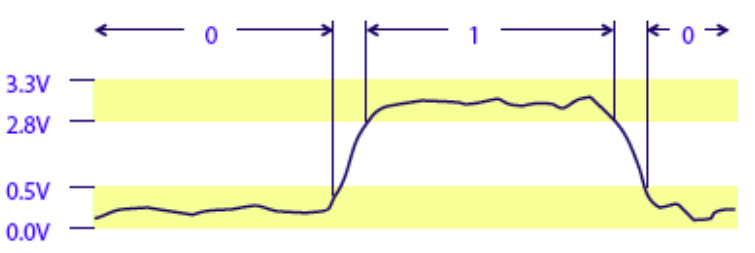
\includegraphics[scale=.5]{images/electric_binary}
\end{center}
\end{figure}

\begin{history}
En 1939, Claude Shannon a été le premier à faire un parallèle entre l'algèbre booléenne (une algèbre binaire, n'acceptant que vrai et faux comme valeurs, et trois fonctions logiques “Et (*), Ou(+), Non(-)”) et le fonctionnement des circuits électriques. Le vrai/faux se transforme en 1 : le courant passe, 0 : il ne passe pas. C'est Shannon qui popularise le terme de bit:
\end{history}

\begin{definition}
Le terme {\bf bit} (b minuscule dans les notations) signifie {\it binary digit }, c'est-à-dire 0 ou 1 en numérotation binaire. Il s'agit de la plus petite unité d'information manipulable par une machine numérique. 


L'{\bf octet} (en anglais {\bf byte} ou B majuscule dans les notations) est une unité d'information composée de 8 bits. Il permet notamment de représenter un caractère, comme une lettre, un chiffre ou un symbole.
\end{definition}

D'autres termes sont aussi utilisés pour définir certaines longueurs de nombres :
\begin{itemize}
\item Un octet est l’unité de base de la mémoire des ordinateurs.
\item Une unité d'information composée de 16 bits est généralement appelée {\bf mot} (en anglais {\bf word}).

\item Une unité d'information de 32 bits de longueur est appelée {\bf mot double} (en anglais {\bf double word}, d'où l'appellation dword).
\end{itemize}
\begin{aretenir}
Toute information traitée par un ordinateur est finalement représentée sous la forme d'une suite de bits (0 et 1).
\end{aretenir}

\section{Les bases décimales, binaires et hexadécimales}


\subsection{La base décimale}

Le système décimal (base 10) est celui que nous utilisons dans la vie quotidienne historiquement liée au fait que l'être humain compte avec ses dix doigts. Il comporte 10 symboles de 0 à 9. C'est un système positionnel, c'est-à-dire que l'endroit où se trouve le symbole définit sa valeur.

Par exemple: $(9'875)_{(10)}=9 \cdot 10^3 + 8 \cdot 10^2 + 7\cdot 10^1 + 5 \cdot 10^0$

10 représente la base et les puissances de 0 à 3 le rang de chaque chiffre. Quelle que soit la base, le chiffre de droite est celui des unités. Celui de gauche est celui qui a le poids le plus élevé.

\subsection{Binaire}

Dans les domaines de l'automatisme, de l'électronique et de l'informatique, nous utilisons la base 2. Tous les nombres sont représentés uniquement à l'aide des chiffres 0 et 1.  Car l'algèbre booléenne est à la base de l'électronique numérique. Par exemple, un interrupteur est ouvert ou fermé, une diode électroluminescente (ou LED en anglais) est allumée ou éteinte,  une tension est présente ou absente, un champ magnétique est orienté Nord-Sud ou Sud-Nord.

Le chiffre binaire, qui peut prendre ces deux états, est nommé {\bf bit} (binary digit). Les règles sont les mêmes que pour le décimal. 

Par exemple, $1101_{(2)}=1 \cdot 2^3 + 1 \cdot 2^2 + 0 \cdot 2^1 + 1\cdot 2^0=13_{(10)}$ 

\subsubsection{Compter en binaire}
Comptons en binaire pour voir comment ça fonctionne.

\begin{center}
\renewcommand{\arraystretch}{1.25}
\begin{tabular}{l*{11}{c}}

\textbf{Décimal} & 0 & 1 & 2 & 3 & 4 & 5 & 6 & 7 & 8 & 9 & 10 \\
\cmidrule(lr){1-12}
\rowcolor{gray!10}
\textbf{Binaire} & 0 & 1 & 10 & 11 & 100 & 101 & 110 & 111 & 1000 & 1001 & 1010 \\

\end{tabular}
\end{center}

Entrons dans le détail pour comprendre comment convertir des nombres binaires et des nombres décimaux et inversement.
\subsubsection{Conversion binaire décimale}

Une méthode pour obtenir le nombre en base 10, connaissant son écriture en base 2, est d'établir la valeur de chaque chiffre du nombre: celui le plus à droite représente 1, le deuxième représente 2, le troisième représente $2^2=4$, le quatrième représente $2^3=8$, etc. comme dans la grille ci-dessous :  

\begin{center}
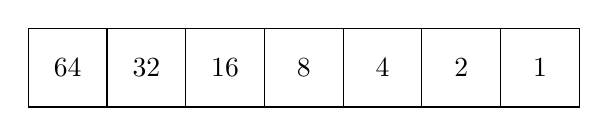
\begin{tikzpicture}
	\draw (-1,1) rectangle (0,0) rectangle (1,1) rectangle (2,0) rectangle (3,1) rectangle (4,0) rectangle (5,1) rectangle (6,0);
	\draw (5.5,0.5) node {$1$};
	\draw (4.5,0.5) node {$2$};
	\draw (3.5,0.5) node {$4$};
	\draw (2.5,0.5) node {$8$};
	\draw (1.5,0.5) node {$16$};
	\draw (0.5,0.5) node {$32$};
	\draw (-.5,0.5) node {$64$};
	
\end{tikzpicture}
\end{center} 

Par exemple, si nous voulons connaître la valeur décimale du nombre 10110, nous établissons d'abord une grille avec les différentes puissances de 2; ensuite, nous plaçons le nombre en binaire sous cette grille en mettant bien le chiffre des unités sous le carré le plus à droite:

\begin{center}
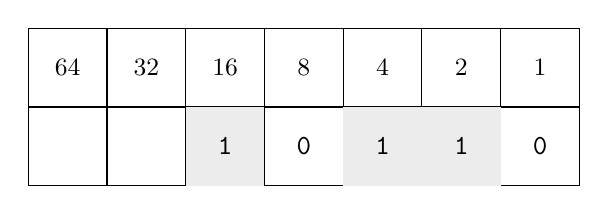
\begin{tikzpicture}[font=\small]
\def\cell{1}

% Grille
\draw[line width=0.4pt] (0,0) grid (7,2);

% Cases actives
\foreach \x in {2,4,5}
{
    \fill[gray!15] (\x,0) rectangle ++(1,1);
}

% Valeurs
\foreach \x/\val in {
0/64,1/32,2/16,3/8,4/4,5/2,6/1}
{
    \node at (\x+0.5,1.5) {\val};
}

% Bits
\foreach \x/\bit in {
0/{},1/{},2/1,3/0,4/1,5/1,6/0}
{
    \node[font=\ttfamily] at (\x+0.5,0.5) {\bit};
}

\end{tikzpicture}
\end{center}

Il ne reste plus qu'à additionner les nombres des colonnes qui contiennent un 1: $16 + 4 + 2=22$

N.B. : Ce tableau est extensible à l'infini vers la gauche avec les puissances de 2 suivantes.

\begin{exercice}
\'Ecrire en base 10 les nombres suivants:
\begin{multicols}{2}
\begin{enumerate}
\item $101_{(2)}$ 
\item $10 000_{(2)}$
\item $1111_{(2)}$
\item $10101_{(2)}$
\item $10_{(2)}$
\item $111 000_{(2)}$

\end{enumerate}
\end{multicols}

Vous pouvez utiliser le tableau ci-dessous : 

\begin{center}
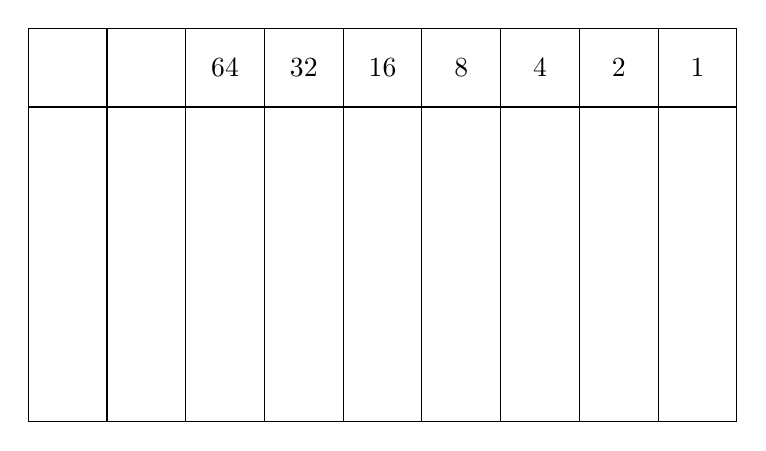
\begin{tikzpicture}
	\draw (-3,1) rectangle (-2,0) rectangle (-1,1) rectangle (0,0) rectangle (1,1) rectangle (2,0) rectangle (3,1) rectangle (4,0) rectangle (5,1) rectangle (6,0);
	\draw (5.5,0.5) node {$1$};
	\draw (4.5,0.5) node {$2$};
	\draw (3.5,0.5) node {$4$};
	\draw (2.5,0.5) node {$8$};
	\draw (1.5,0.5) node {$16$};
	\draw (0.5,0.5) node {$32$};
	\draw (-.5,0.5) node {$64$};
	\draw (-3,-4) rectangle (-2,0) rectangle (-1,-4) rectangle (0,0) rectangle (1,-4) rectangle (2,0) rectangle (3,-4) rectangle (4,0) rectangle (5,-4) rectangle (6,0);
	
\end{tikzpicture}
\end{center} 

\end{exercice}

\subsubsection{Conversion décimale binaire}

Pour trouver l'écriture binaire d'un nombre écrit en base 10, il existe principalement deux méthodes. 


\; 

La première méthode consiste à décomposer le nombre en somme de puissance de 2 et à utiliser la grille précédente. 

Plus concrètement, si nous voulons écrire 99 en binaire. La plus grande puissance de 2 que nous pouvons prendre dans 99 est 64 (128, la suivante, est trop grande). Il reste ensuite: 

99 - \textbf{64} = 35. Dans 35 on peut mettre 32, et il restera 

35 - \textbf{32} = 3. Dans 3 on ne peut ni mettre 16, ni mettre 8, ni mettre 4. On peut mettre 2 :

3 - \textbf{2} = 1. Il reste 1 et dans 1 on peut mettre 1 :

1 - \textbf{1} = 0

Cela signifie que 99 = 64 + 32 + 2 + 1. Sur notre grille cela donne:

\begin{center}
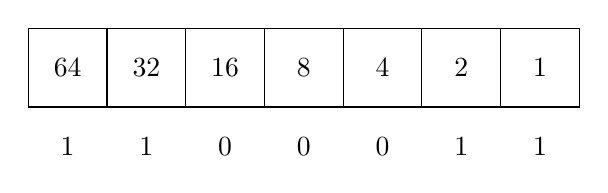
\begin{tikzpicture}
	\draw (-1,1) rectangle (0,0) rectangle (1,1) rectangle (2,0) rectangle (3,1) rectangle (4,0) rectangle (5,1) rectangle (6,0);
	\draw (5.5,0.5) node {$1$};
	\draw (4.5,0.5) node {$2$};
	\draw (3.5,0.5) node {$4$};
	\draw (2.5,0.5) node {$8$};
	\draw (1.5,0.5) node {$16$};
	\draw (0.5,0.5) node {$32$};
	\draw (-.5,0.5) node {$64$};
	
	\draw (5.5,-0.5) node {$1$};
	\draw (4.5,-0.5) node {$1$};
	\draw (3.5,-0.5) node {$0$};
	\draw (2.5,-0.5) node {$0$};
	\draw (1.5,-0.5) node {$0$};
	\draw (0.5,-0.5) node {$1$};
	\draw (-.5,-0.5) node {$1$};
	
%	\draw (1,0) -- +(1,1)
%				(2,0) -- +(1,1)
%				(3,0) -- +(1,1)
%				;
	
\end{tikzpicture}
\end{center}

Donc $99_{(10)}=1100011_{(2)}$.


\;

La deuxième méthode consiste  à effectuer des divisions successives par 2. Le nombre en binaire se lira à l'aide des restes des différentes divisions:

\begin{figure}[h]
\begin{center}
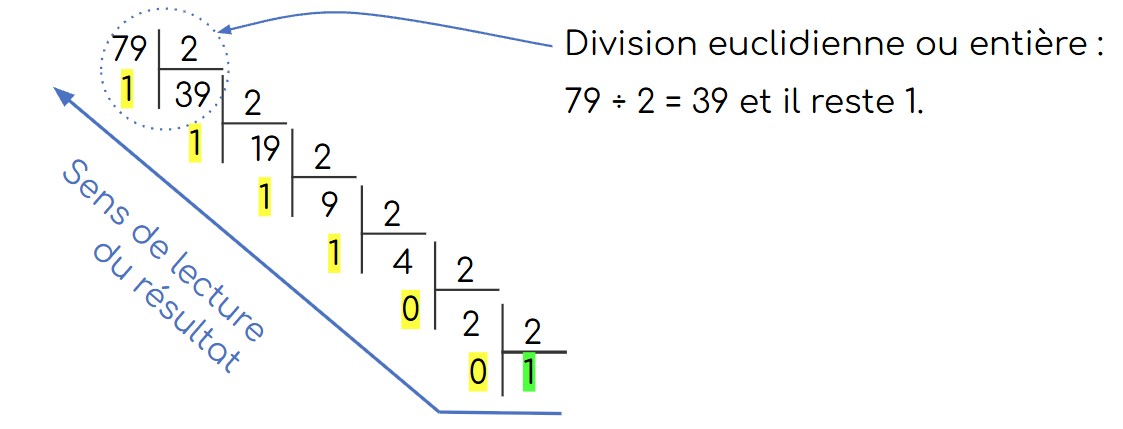
\includegraphics[scale=.6]{images/divisionbinaire}
\end{center}
\end{figure}

Ainsi, $79_{(10)}=1001111_{(2)}$

\begin{exercice}
Les nombres suivants sont écrits en base 10. Donner leur écriture en base 2:
\begin{multicols}{2}
\begin{enumerate}
\item 75
\item 12
\item 27
\item 153
\item 100
\item 200
\item 1000
\item 2000
\end{enumerate}
\end{multicols}
\end{exercice}



\subsection{Opération sur les nombres en binaires}

Tout comme pour l'addition en colonne, pour additionner deux nombres écrits en binaire, il faut les additionner bit à bit. 
\filbreak
\begin{exercice}
Quel est le résultat des calculs binaires suivants:
\begin{enumerate}
\item $0+0=$
\ 

\item $1+0=$
\ 

\item $0+1=$
\ 

\item $1+1=$
\ 

\item $1+1+1=$
\end{enumerate}
\end{exercice}

À l'aide de l'exercice suivant, effectuer l'addition suivante :

$$1100101001 + 101110101$$

Pour cela, compléter l'addition en colonne suivante:

\;

\begin{center}
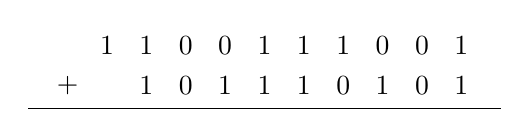
\begin{tikzpicture}
	\draw (0,0) node{$1$}
				(0.5,0) node{$1$}
				(1,0) node{$0$}
				(1.5,0) node{$0$}
				(2,0) node{$1$}
				(2.5,0) node{$1$}
				(3,0) node{$1$}
				(3.5,0) node{$0$}
				(4,0) node{$0$}
				(4.5,0) node{$1$};
		\draw (-0.5,-.5) node{$+$}
				(0.5,-.5) node{$1$}
				(1,-.5) node{$0$}
				(1.5,-.5) node{$1$}
				(2,-.5) node{$1$}
				(2.5,-.5) node{$1$}
				(3,-.5) node{$0$}
				(3.5,-.5) node{$1$}
				(4,-.5) node{$0$}
				(4.5,-.5) node{$1$};
	\draw (-1,-.8) -- +(6,0);
\end{tikzpicture}
\end{center}

\vskip+1cm

\begin{aretenir}
Toujours être attentif à la base: $1_{(2)} + 1_{(2)} = 10_{(2)} \qquad \text{alors que} \qquad  1_{(10)} + 1_{(10)} = 2_{(10)}$
\end{aretenir}

\begin{exercice}
Effectuer les additions binaires suivantes:
\begin{multicols}{2}
\begin{enumerate}
\item $1001 + 101$
\item $10011 + 110011$
\item  $110001 + 11010$
\item $110101 + 101110$
\end{enumerate}
\end{multicols}
\end{exercice}


\begin{exercice}
\begin{enumerate}
\item On voudrait encoder des emojis en binaire; en d'autres mots, on voudrait faire correspondre chaque emoji à un code binaire différent.
\begin{enumerate}
\item Combien peut-on encoder de symboles (ici des emojis) différents sur 3 bits ?
\item Sur 5 bits ?
\item Sur 11 bits ?
\end{enumerate}

\item Combien de nombres peut-on représenter avec 5 bits et avec 12 bits ?

\item Quel est le plus grand nombre qu'on peut écrire sur 8 bits ?


\vspace{10pt}
\item On se pose maintenant la question inverse : 
\begin{enumerate}
\item Combien me faut-il de bits pour encoder 8 symboles différents ?
\item 9 symboles ?
\item 69 symboles ?
\end{enumerate}

\end{enumerate}
\end{exercice}

\subsection{*La base hexadécimale}

C'est le code utilisé dans la programmation de certains automates et microprocesseurs. Il est composé de : 10 chiffres de 0 à 9, et 6 lettres de A à F. Les adresses MAC (adresses uniques associées à chaque carte réseau dans le monde) sont aussi écrites en base hexadécimale.

La manipulation des nombres écrits en binaire est difficile pour l'être humain et la conversion en décimal n'est pas simple. C'est pourquoi nous utilisons de préférence le système hexadécimal (base 16). 

Le tableau ci-dessous montre la représentation des nombres de 0 à 15 dans les bases 10, 2 et 16.

\begin{figure}[h]
\begin{center}
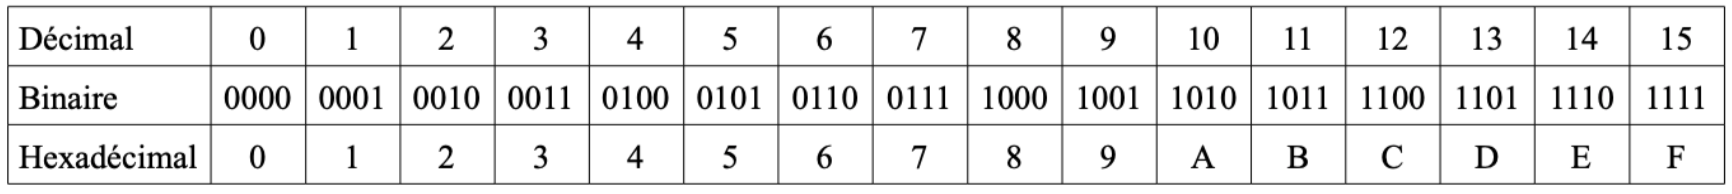
\includegraphics[scale=.5]{images/tableaubase}
\end{center}
\end{figure}


Par exemple, $B4F_{(16)}= B \cdot 16^2 + 4 \cdot 16^1 + F\cdot 16^0= 11 \cdot 16^2 + 4 \cdot 16^1 + 15\cdot 16^0=2\,895_{(10)}$

\subsubsection{Conversion en binaire}

Pour convertir un nombre binaire en hexadécimal il suffit de remarquer que chaque groupe de 4 bits représente un chiffre en hexadécimal:

\begin{figure}[h]
\begin{center}
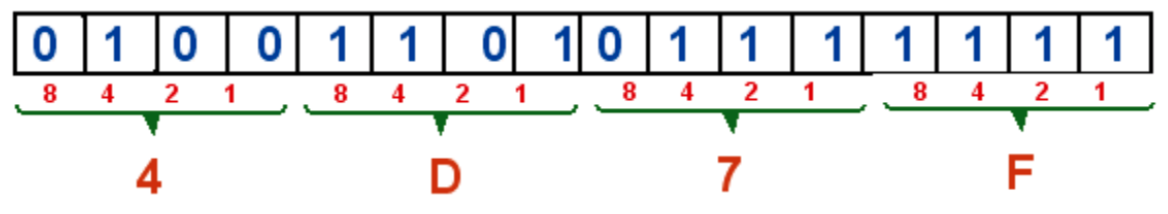
\includegraphics[scale=.5]{images/hexadecimal}
\end{center}
\end{figure}

\begin{exercice}
* Écrire les nombres suivants en base hexadécimale:
\begin{multicols}{2}
\begin{enumerate}
\item $10010010110_{(2)}$
\item $111110_{(2)}$
\item  $1000110101110101_{(2)}$
\item $11110000000011_{(2)}$
\end{enumerate}
\end{multicols}
\end{exercice}



\subsubsection{Conversion en décimal}

La méthode par division (par 16) s'applique comme en binaire (par 2).

\begin{exercice}
* Écrire les nombres suivants en hexadécimal:
\begin{multicols}{2}
\begin{enumerate}
\item 92
\item 256
\item  500
\item 1023
\end{enumerate}
\end{multicols}
\end{exercice}

\section{Représentation des nombres entiers relatifs signés}

\begin{definition}
Les \textbf{nombres entiers naturels} sont les nombres entiers positifs ou nuls :
    \[
        \mathbb{N}=\{0,1,2,3,\ldots\}
    \]

Les \textbf{nombres entiers relatifs} regroupent les nombres entiers
    négatifs, le nombre zéro et les nombres entiers positifs :
    \[
        \mathbb{Z}=\{\ldots,-3,-2,-1,0,1,2,3,\ldots\}
    \]

\end{definition}

Jusqu'à présent, nous avons appris à représenter en binaire des nombres
entiers naturels. Pourtant, de nombreuses situations nécessitent également
des nombres négatifs : une température de $-8\,^\circ$C, un solde bancaire
de $-150$ CHF ou une altitude située sous le niveau de la mer.

Un ordinateur doit donc être capable de représenter aussi bien les nombres
positifs que les nombres négatifs.

\begin{remarque}
Contrairement aux mathématiques, un ordinateur dispose d'une quantité de
mémoire limitée. Chaque nombre doit donc être représenté sur un
\textbf{nombre de bits fixé à l'avance}.

Par exemple, si l'on utilise un octet, chaque nombre occupe exactement
8 bits :

\begin{center}
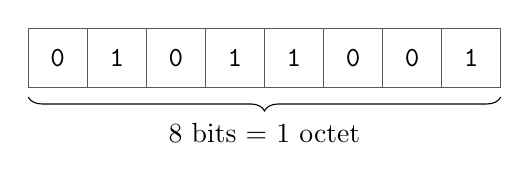
\begin{tikzpicture}[
    bit/.style={
        draw=black!65,
        line width=0.35pt,
        minimum width=0.75cm,
        minimum height=0.75cm,
        inner sep=0pt,
        font=\ttfamily
    }
]
    \foreach \x/\b in {
        0/0,1/1,2/0,3/1,4/1,5/0,6/0,7/1
    }{
        \node[bit] at (\x*0.75,0) {\b};
    }

    \draw[decorate,
          decoration={brace,amplitude=5pt,mirror}]
          (-0.375,-0.5) -- (5.625,-0.5)
          node[midway,below=6pt]{8 bits = 1 octet};
\end{tikzpicture}
\end{center}

En représentation non signée sur 8 bits, le plus petit nombre est
\[
      00000000_{(2)} = 0
\]
et le plus grand est
\[
    11111111_{(2)} = 255
\]
\end{remarque}

\textbf{Problème :} cette représentation ne permet pas d'écrire des nombres
négatifs. Il faut donc définir une convention indiquant comment interpréter
les bits.

\subsection{Représentation signe-magnitude}

Une première idée consiste à réserver le bit situé tout à gauche pour
indiquer le signe du nombre. Ce bit est appelé le \textbf{bit de signe} :

\begin{itemize}
    \item un bit de signe égal à \texttt{0} indique un nombre positif ou nul ;
    \item un bit de signe égal à \texttt{1} indique un nombre négatif ;
    \item les autres bits indiquent la valeur absolue du nombre.
\end{itemize}

\begin{center}
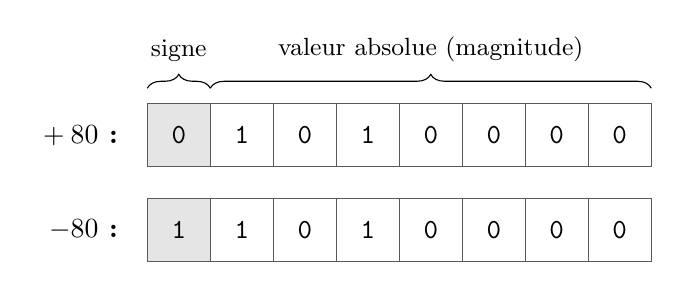
\begin{tikzpicture}[
    bit/.style={
        draw=black!65,
        line width=0.35pt,
        minimum width=0.8cm,
        minimum height=0.8cm,
        inner sep=0pt,
        font=\ttfamily
    }
]
    % Première ligne
    \node[bit,fill=gray!20] at (0,0.6) {0};
    \foreach \x/\b in {
        1/1,2/0,3/1,4/0,5/0,6/0,7/0
    }{
        \node[bit] at (\x*0.8,0.6) {\b};
    }
    \node[anchor=east,font=\bfseries] at (-0.65,0.6) {${}+80$ :};

    % Deuxième ligne
    \node[bit,fill=gray!20] at (0,-0.6) {1};
    \foreach \x/\b in {
        1/1,2/0,3/1,4/0,5/0,6/0,7/0
    }{
        \node[bit] at (\x*0.8,-0.6) {\b};
    }
    \node[anchor=east,font=\bfseries] at (-0.65,-0.6) {$-80$ :};

    % Légendes
    \draw[decorate,
          decoration={brace,amplitude=5pt}]
          (-0.4,1.2) -- (0.4,1.2)
          node[midway,above=6pt]{\small signe};

    \draw[decorate,
          decoration={brace,amplitude=5pt}]
          (0.4,1.2) -- (6.0,1.2)
          node[midway,above=6pt]{\small valeur absolue (magnitude)};
\end{tikzpicture}
\end{center}

Dans cet exemple, la valeur absolue $80$ est représentée par
\[
    1010000_{(2)}.
\]

On ajoute ensuite le bit de signe :

\[
01010000_{(2)} = +80
\]
\[
11010000_{(2)} = -80
\]

Sur 8 bits, un bit est réservé au signe et les 7 autres bits servent à coder
la valeur absolue. On peut donc représenter les nombres compris entre
$-127$ et $+127$ :

\[
    -127 \leqslant x \leqslant 127.
\]

Le plus grand nombre positif est

\[
    \texttt{01111111}_2=+127,
\]

et le plus petit nombre négatif est

\[
    \texttt{11111111}_2=-127.
\]

\subsubsection{Limites de la représentation signe-magnitude}

Cette méthode est simple à comprendre, mais elle présente deux problèmes
importants.

\paragraph{Premier problème : deux représentations du zéro}

\[
\begin{array}{rcl}
\texttt{00000000} &=& +0,\\
\texttt{10000000} &=& -0.
\end{array}
\]

Il existe donc deux suites de bits différentes pour représenter le même
nombre.

\paragraph{Deuxième problème : les additions sont compliquées}

Considérons les représentations signe-magnitude de $+5$ et de $-5$ :

\[
\begin{array}{rcl}
+5 &=& \texttt{00000101},\\
-5 &=& \texttt{10000101}.
\end{array}
\]

Une addition binaire ordinaire donne :

\[
\begin{array}{r@{\;}*{8}{c}}
  & 0&0&0&0&0&1&0&1\\
+ & 1&0&0&0&0&1&0&1\\
\hline
  & 1&0&0&0&1&0&1&0
\end{array}
\]

Le résultat obtenu n'est pas zéro. Il faudrait donc construire des circuits
capables de traiter séparément le signe et la valeur absolue.

Autres exemples:
\begin{figure}[h]
\begin{center}
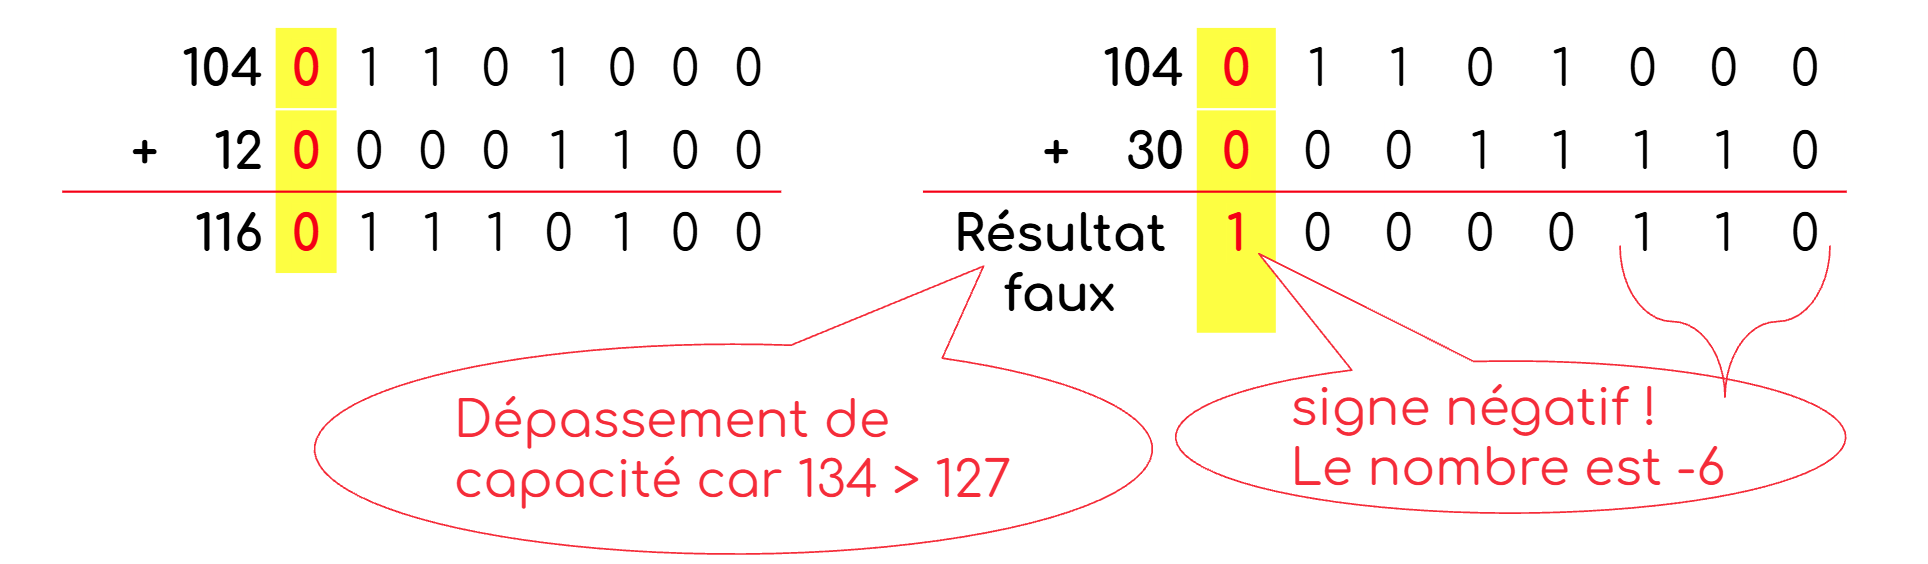
\includegraphics[scale=.4]{images/Operationsigne}
\end{center}
\end{figure}

Pour éviter ces difficultés, les ordinateurs utilisent généralement une
autre représentation : le \textbf{complément à deux}.

\subsection{Représentation en complément à deux*}

\subsubsection{Principe}

Le complément à deux est la méthode habituellement utilisée pour représenter
les nombres entiers relatifs dans un ordinateur.

Avec cette représentation :

\begin{itemize}
    \item les nombres positifs et le nombre zéro sont écrits normalement en
    binaire ;
    \item les nombres négatifs sont codés selon une règle particulière ;
    \item le nombre zéro ne possède qu'une seule représentation ;
    \item les additions peuvent être réalisées avec le même circuit, que les
    nombres soient positifs ou négatifs.
\end{itemize}

Sur $n$ bits, le complément à deux permet de représenter les nombres compris
entre

\[
    -2^{n-1}
    \qquad\text{et}\qquad
    2^{n-1}-1.
\]

Par exemple, sur 8 bits :

\[
    -2^7 \leqslant x \leqslant 2^7-1,
\]

c'est-à-dire

\[
    -128 \leqslant x \leqslant 127.
\]

\subsubsection{Comment représenter un nombre négatif ?}

Pour écrire un nombre négatif en complément à deux, on applique trois étapes :

\begin{enumerate}
    \item écrire sa valeur positive en binaire sur le nombre de bits choisi ;
    \item inverser tous les bits : les \texttt{0} deviennent des \texttt{1}
    et les \texttt{1} deviennent des \texttt{0} ;
    \item ajouter \texttt{1} au résultat.
\end{enumerate}

Prenons comme exemple la représentation de $-80$ sur 8 bits.

\begin{center}
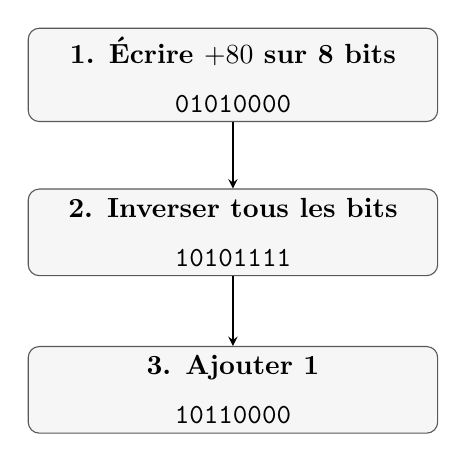
\begin{tikzpicture}[
    étape/.style={
        rounded corners,
        draw=black!65,
        line width=0.4pt,
        fill=gray!7,
        minimum width=5.2cm,
        minimum height=1.1cm,
        align=center
    },
    flèche/.style={
        ->,
        >=stealth,
        line width=0.5pt
    }
]
    \node[étape] (a) at (0,0)
        {\textbf{1. Écrire $+80$ sur 8 bits}\\[2mm]
         \texttt{01010000}};

    \node[étape] (b) at (0,-2)
        {\textbf{2. Inverser tous les bits}\\[2mm]
         \texttt{10101111}};

    \node[étape] (c) at (0,-4)
        {\textbf{3. Ajouter 1}\\[2mm]
         \texttt{10110000}};

    \draw[flèche] (a) -- (b);
    \draw[flèche] (b) -- (c);
\end{tikzpicture}
\end{center}

Ainsi, la représentation de $-80$ en complément à deux sur 8 bits est

\[
    \boxed{\texttt{10110000}}.
\]

\begin{remarque}
Pour obtenir l'opposé d'un nombre en complément à deux, on peut appliquer
exactement la même procédure : inverser tous les bits, puis ajouter 1.

Cette méthode permet donc de passer de $+80$ à $-80$, mais également de
$-80$ à $+80$.
\end{remarque}

\subsubsection{Vérification par une addition}

L'un des principaux avantages du complément à deux est que les additions
binaires fonctionnent normalement, même lorsque l'un des nombres est
négatif.

Vérifions que

\[
    80+(-80)=0.
\]

Les deux nombres sont représentés sur 8 bits par

\[
\begin{array}{rcl}
+80 &=& \texttt{01010000},\\
-80 &=& \texttt{10110000}.
\end{array}
\]

Effectuons l'addition :

\[
\begin{array}{r@{\;}*{9}{c}}
  &   &0&1&0&1&0&0&0&0\\
+ &   &1&0&1&1&0&0&0&0\\
\hline
  & 1&0&0&0&0&0&0&0&0
\end{array}
\]

Le calcul produit 9 bits :

\[
    \texttt{1 00000000}.
\]

Or les nombres sont codés sur seulement 8 bits. Le bit supplémentaire situé
tout à gauche est donc ignoré. Il reste :

\[
    \texttt{00000000}=0.
\]

On obtient bien

\[
    80+(-80)=0.
\]

\subsubsection{Comment lire un nombre négatif ?}

Dans une représentation en complément à deux, le bit situé tout à gauche
permet de déterminer le signe :

\begin{itemize}
    \item s'il vaut \texttt{0}, le nombre est positif ou nul ;
    \item s'il vaut \texttt{1}, le nombre est négatif.
\end{itemize}

Pour retrouver la valeur d'un nombre négatif, on applique de nouveau la
procédure du complément à deux.

Prenons le nombre

\[
    \texttt{11111011}.
\]

Son bit de gauche vaut \texttt{1} : le nombre est donc négatif.

\begin{enumerate}
    \item On inverse tous les bits :
    \[
        \texttt{00000100}.
    \]

    \item On ajoute 1 :
    \[
        \texttt{00000101}=5.
    \]
\end{enumerate}

La suite de bits initiale représente donc

\[
    \texttt{11111011}=-5.
\]

\subsubsection{Quelques valeurs sur 4 bits}

Sur 4 bits, on peut représenter les nombres compris entre

\[
    -2^3=-8
    \qquad\text{et}\qquad
    2^3-1=7.
\]

\begin{center}
\renewcommand{\arraystretch}{1.2}
\begin{tabular}{ccc}
\toprule
\textbf{Binaire} & \textbf{Valeur décimale} & \textbf{Signe} \\
\midrule
\texttt{0000} & 0  & positif ou nul \\
\texttt{0001} & 1  & positif \\
\texttt{0010} & 2  & positif \\
\texttt{0011} & 3  & positif \\
\texttt{0100} & 4  & positif \\
\texttt{0101} & 5  & positif \\
\texttt{0110} & 6  & positif \\
\texttt{0111} & 7  & positif \\
\midrule
\texttt{1000} & $-8$ & négatif \\
\texttt{1001} & $-7$ & négatif \\
\texttt{1010} & $-6$ & négatif \\
\texttt{1011} & $-5$ & négatif \\
\texttt{1100} & $-4$ & négatif \\
\texttt{1101} & $-3$ & négatif \\
\texttt{1110} & $-2$ & négatif \\
\texttt{1111} & $-1$ & négatif \\
\bottomrule
\end{tabular}
\end{center}

On remarque que :

\[
\begin{array}{rcl}
\texttt{0111} &=& +7,\\
\texttt{1000} &=& -8,\\
\texttt{1111} &=& -1,\\
\texttt{0000} &=& 0.
\end{array}
\]

\begin{remarque}
En complément à deux, il y a une valeur négative de plus que de valeurs
strictement positives.

Sur 8 bits, l'intervalle va de $-128$ à $+127$.
\end{remarque}

\subsection{Comparaison des représentations}

\begin{center}
\renewcommand{\arraystretch}{1.3}
\begin{tabularx}{\textwidth}{lCCC}
\toprule
\textbf{Représentation}
&
\textbf{Deux zéros}
&
\textbf{Additions simples}
&
\textbf{Usage courant}
\\
\midrule
Non signée
&
---
&
Oui
&
Pour les entiers naturels
\\

Signe-magnitude
&
Oui
&
Non
&
Rare
\\

Complément à deux
&
Non
&
Oui
&
Entiers relatifs
\\
\bottomrule
\end{tabularx}
\end{center}

\subsection{Résumé}

\begin{aretenir}
\begin{itemize}
\renewcommand{\labelitemi}{$\bullet$}

    \item Une suite de bits n'a pas de signification unique : son
    interprétation dépend de la représentation choisie.

    \item En représentation non signée sur $n$ bits, les valeurs vont de
    $0$ à $2^n-1$.

    \item En représentation signe-magnitude, le bit de gauche indique le
    signe et les autres bits représentent la valeur absolue.

    \item La représentation signe-magnitude possède deux zéros et complique
    les opérations arithmétiques.

    \item Le complément à deux est la méthode habituellement utilisée par les
    ordinateurs pour représenter les nombres entiers relatifs.

    \item Pour écrire l'opposé d'un nombre en complément à deux, on inverse
    tous les bits, puis on ajoute 1.

    \item Sur $n$ bits, les valeurs en complément à deux vont de
    $-2^{n-1}$ à $2^{n-1}-1$.
\end{itemize}
\end{aretenir}

\begin{exercice}
En supposant que les nombres soient écrits sur 8 bits :

\begin{enumerate}
    \item écrire $+5$ en binaire ;
    \item déterminer la représentation de $-5$ en complément à deux ;
    \item effectuer l'addition $5+(-5)$ ;
    \item expliquer pourquoi le résultat obtenu représente bien zéro.
\end{enumerate}
\end{exercice}

\begin{exercice}
Donner la représentation signe-magnitude sur un octet des nombres suivants.
Lorsqu'un nombre ne peut pas être représenté, expliquer pourquoi.

\begin{multicols}{2}
\begin{enumerate}
    \item $-100$
    \item $38$
    \item $-200$
    \item $-83$
\end{enumerate}
\end{multicols}
\end{exercice}

\begin{exercice}
\textbf{*Complément à deux}

Tous les nombres sont codés sur 8 bits.

\begin{enumerate}
    \item Donner la représentation en complément à deux des nombres suivants :
    \begin{enumerate}
        \item $-95$
        \item $-64$
    \end{enumerate}

    \item Vérifier que $95+(-95)$ donne bien zéro.

    \item Représenter $-6$ en complément à deux, puis vérifier que
    \[
        64+(-6)=58.
    \]

    \item Vérifier que la représentation binaire de $58$ sur 8 bits est
    \[
        \texttt{00111010}.
    \]
\end{enumerate}
\end{exercice}

\begin{exercice}
Pour chacune des suites de 8 bits suivantes :

\[
\begin{array}{lll}
\text{a) }\texttt{00101010}
&
\text{b) }\texttt{00001011}
&
\text{c) }\texttt{10111111}
\end{array}
\]

déterminer sa valeur :

\begin{enumerate}
    \item en représentation non signée ;
    \item en représentation signe-magnitude ;
    \item en représentation en complément à deux.
\end{enumerate}

Que peut-on conclure sur la signification d'une suite de bits ?
\end{exercice}

\section{Les codes de caractères}

Nous savons maintenant représenter des nombres à l'aide de bits. Mais un ordinateur
ne manipule pas uniquement des nombres : il doit également pouvoir stocker et
transmettre du texte.

Par exemple, lorsque nous appuyons sur la touche \texttt{A} du clavier, l'ordinateur
doit pouvoir représenter ce caractère sous forme numérique.

\begin{aretenir}
Un ordinateur ne stocke donc pas directement les lettres ou les symboles.
Il leur associe des \textbf{nombres}, qui sont ensuite représentés en binaire.

Un \textbf{code de caractères} définit la correspondance entre les caractères
et ces nombres.
\end{aretenir}


\subsection{La table ASCII}

L'un des premiers standards largement utilisés pour représenter du texte est le
code \textbf{ASCII} (\textit{American Standard Code for Information Interchange}),
publié dans les années 1960.

ASCII utilise \textbf{7 bits}. Il permet donc de représenter

\[
2^7 = 128
\]

valeurs différentes, numérotées de 0 à 127.

Chaque caractère est associé à un nombre. Par exemple :

\begin{center}
\renewcommand{\arraystretch}{1.25}
\begin{tabular}{cccc}
\toprule
\textbf{Caractère} & \textbf{ASCII décimal} & \textbf{Binaire} & \textbf{Hexadécimal} \\
\midrule
\texttt{A} & 65  & \texttt{01000001} & \texttt{41} \\
\texttt{B} & 66  & \texttt{01000010} & \texttt{42} \\
\texttt{a} & 97  & \texttt{01100001} & \texttt{61} \\
\texttt{f} & 102 & \texttt{01100110} & \texttt{66} \\
\texttt{2} & 50  & \texttt{00110010} & \texttt{32} \\
\texttt{?} & 63  & \texttt{00111111} & \texttt{3F} \\
\texttt{espace} & 32 & \texttt{00100000} & \texttt{20} \\
\bottomrule
\end{tabular}
\end{center}

Par exemple, le caractère \texttt{A} possède le code ASCII 65. En binaire :

\[
\texttt{A}
\quad\longrightarrow\quad
65
\quad\longrightarrow\quad
\texttt{01000001}
\]

\begin{aretenir}
Le caractère \texttt{2} et le nombre $2$ ne doivent pas être confondus.

Le nombre $2$, utilisé dans un calcul, peut être représenté en binaire par
\texttt{00000010}.

Le caractère \texttt{2}, utilisé dans un texte, possède le code ASCII 50 et est
donc représenté par \texttt{00110010}.
\end{aretenir}

\subsubsection{Organisation de la table ASCII}

Les 128 codes ASCII sont organisés en plusieurs groupes :

\begin{itemize}
    \item les codes \textbf{0 à 31}, ainsi que le code 127, sont principalement
    des \textbf{caractères de contrôle} ;

    \item les codes \textbf{32 à 126} correspondent aux caractères affichables :
    lettres, chiffres, signes de ponctuation et symboles ;

    \item les lettres majuscules \texttt{A} à \texttt{Z} occupent les codes
    \textbf{65 à 90} ;

    \item les lettres minuscules \texttt{a} à \texttt{z} occupent les codes
    \textbf{97 à 122} ;

    \item les chiffres \texttt{0} à \texttt{9} occupent les codes
    \textbf{48 à 57}.
\end{itemize}

Les caractères de contrôle ne représentent généralement pas un symbole visible.
Ils servaient notamment à commander les terminaux et les périphériques.

Quelques exemples :

\begin{center}
\renewcommand{\arraystretch}{1.2}
\begin{tabular}{ccl}
\toprule
\textbf{Code} & \textbf{Nom} & \textbf{Fonction} \\
\midrule
7  & BEL & signal sonore \\
9  & TAB & tabulation \\
10 & LF  & passage à la ligne suivante \\
13 & CR  & retour au début de la ligne \\
27 & ESC & échappement \\
\bottomrule
\end{tabular}
\end{center}

\begin{center}
\begin{figure}[h!]
\centering
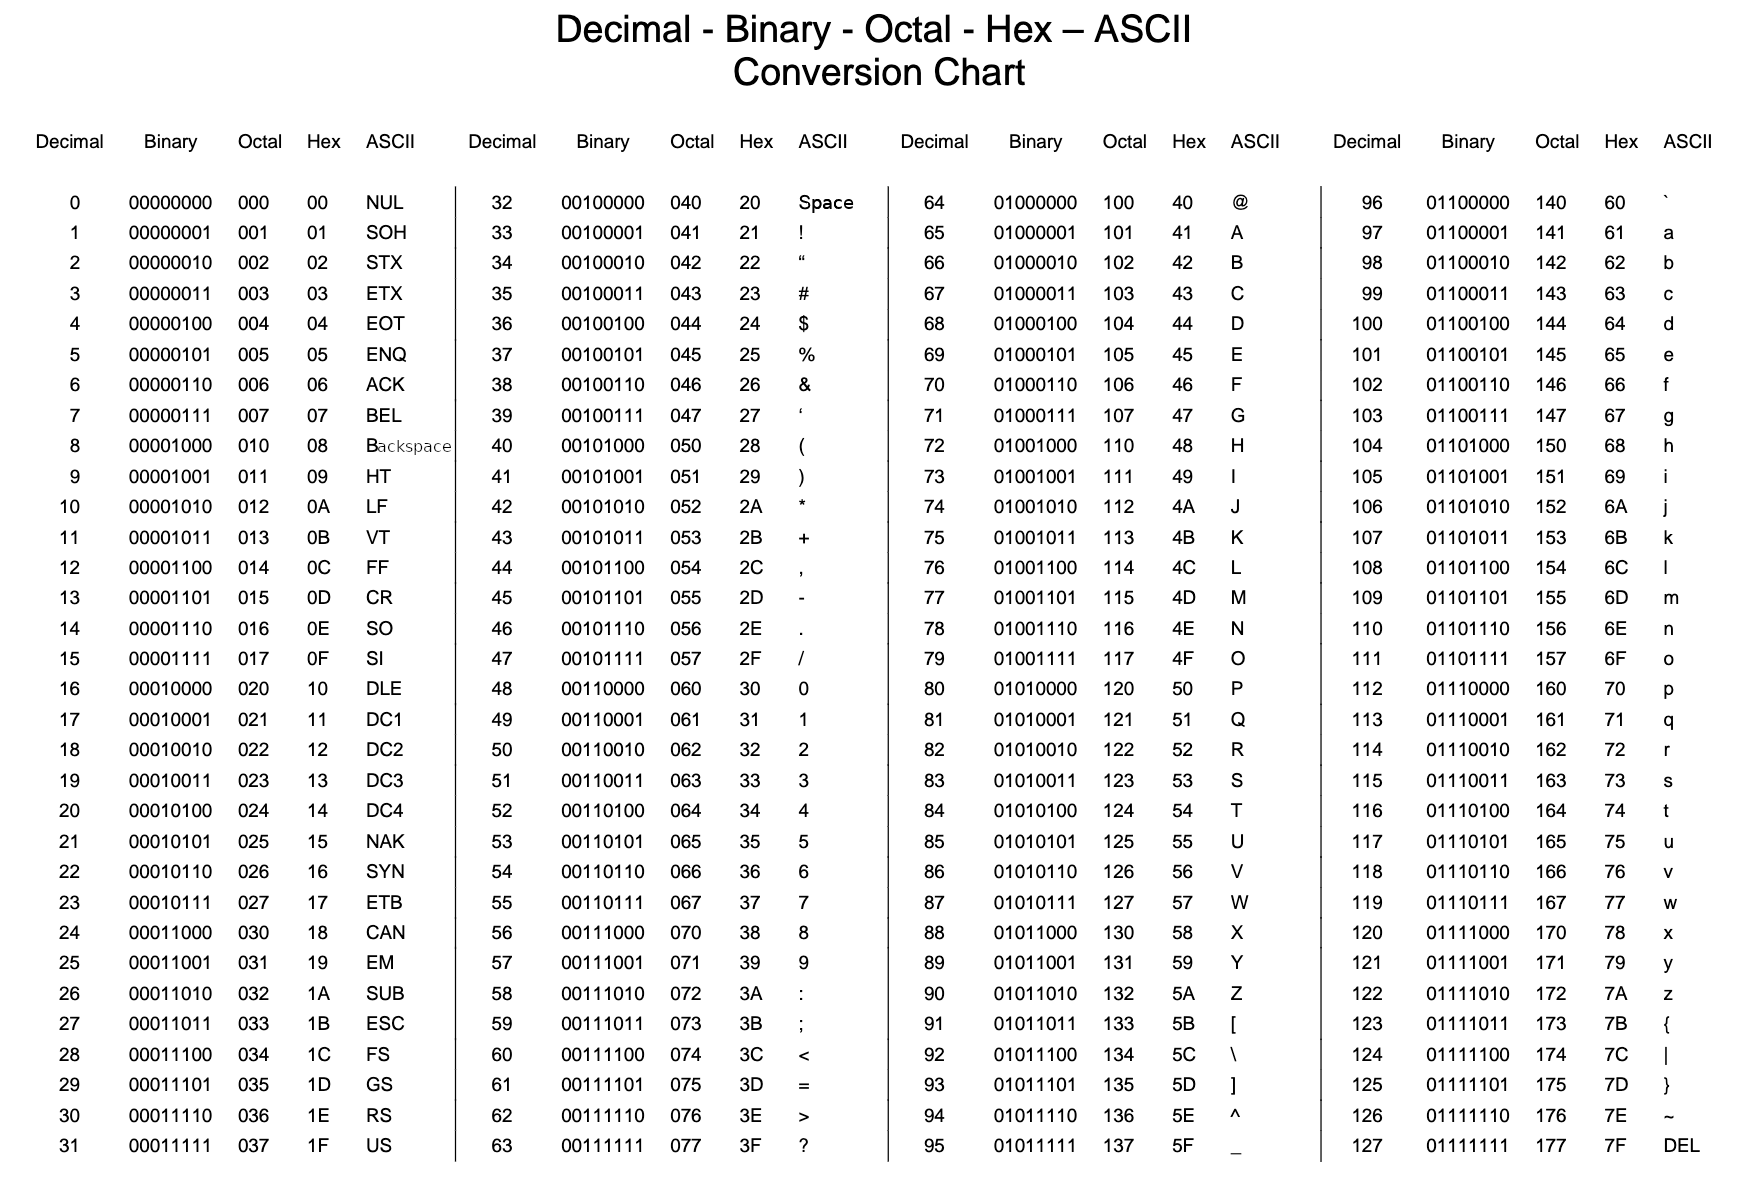
\includegraphics[width=\textwidth]{images/ASCII2}
\caption{Table des caractères ASCII}
\end{figure}
\end{center}


\subsubsection{Les limites d'ASCII}

ASCII a été conçu principalement pour la langue anglaise.

Il permet d'écrire :

\begin{center}
\texttt{Hello world!}
\end{center}

mais il ne contient pas de caractères tels que :

\begin{center}
\texttt{é \qquad è \qquad à \qquad ç \qquad ü}
\end{center}

et encore moins les caractères utilisés dans d'autres systèmes d'écriture :

\begin{center}
\renewcommand{\arraystretch}{1.25}
\begin{tabular}{ccc}
\toprule
\textbf{Caractère} & \textbf{Unicode} & \textbf{Valeur décimale} \\
\midrule
A          & \texttt{U+0041} & 65 \\
é          & \texttt{U+00E9} & 233 \\
$\Omega$   & \texttt{U+03A9} & 937 \\
\bottomrule
\end{tabular}
\end{center}

Pour représenter davantage de caractères, différents systèmes utilisant 8 bits
ont été développés. Ils permettaient de représenter jusqu'à

\[
2^8 = 256
\]

valeurs.

On parle souvent, de manière générale, d'\textbf{ASCII étendu}.

\begin{aretenir}
Il n'existe cependant pas une unique table « ASCII étendu ». Plusieurs jeux de
caractères différents ont existé, par exemple ISO-8859-1 ou Windows-1252.

Un même nombre pouvait donc représenter des caractères différents selon le
système utilisé.
\end{aretenir}

Cette situation posait un problème important pour l'échange international de
documents. Il fallait disposer d'un système commun capable de représenter les
caractères de toutes les langues.

C'est l'objectif d'\textbf{Unicode}.


\subsection{Unicode}

Unicode est un standard international qui attribue un numéro unique à chaque
caractère.

Ce numéro est appelé un \textbf{point de code} (\textit{code point}).

Il est généralement écrit sous la forme :

\[
\texttt{U+XXXX}
\]

Par exemple :

\begin{center}
\renewcommand{\arraystretch}{1.25}
\begin{tabular}{ccc}
\toprule
\textbf{Caractère} & \textbf{Unicode} & \textbf{Valeur décimale} \\
\midrule
\texttt{A} & \texttt{U+0041} & 65 \\
\texttt{é} & \texttt{U+00E9} & 233 \\
$\Omega$   & \texttt{U+03A9} & 937 \\
\bottomrule
\end{tabular}
\end{center}

Unicode permet ainsi de représenter des caractères provenant de très nombreux
systèmes d'écriture : alphabet latin, grec, cyrillique, arabe, hébreu,
caractères chinois, japonais, coréens, etc.

Il permet également de représenter de nombreux symboles et les emoji.

\begin{aretenir}
Unicode est compatible avec ASCII : les 128 premiers points de code Unicode
correspondent aux caractères ASCII.

Ainsi :
\[
\texttt{A}
\quad=\quad
\text{ASCII }65
\quad=\quad
\text{Unicode U+0041}.
\]
\end{aretenir}


\subsection{Unicode et UTF-8}

Il faut distinguer deux notions :

\begin{itemize}
    \item \textbf{Unicode} indique quel numéro est associé à chaque caractère ;

    \item \textbf{UTF-8} indique comment ce numéro est représenté en mémoire
    sous forme d'octets.
\end{itemize}

On peut résumer le processus ainsi :

\begin{center}
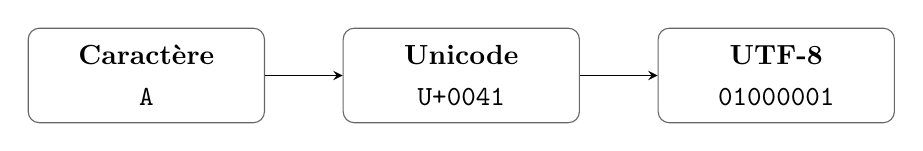
\begin{tikzpicture}[
    box/.style={
        draw=black!60,
        line width=0.4pt,
        rounded corners,
        minimum width=3cm,
        minimum height=1.2cm,
        align=center
    },
    fleche/.style={
        ->,
        >=stealth,
        line width=0.5pt
    }
]

\node[box] (car) at (0,0)
    {\textbf{Caractère}\\[1mm]\texttt{A}};

\node[box] (uni) at (4,0)
    {\textbf{Unicode}\\[1mm]\texttt{U+0041}};

\node[box] (utf) at (8,0)
    {\textbf{UTF-8}\\[1mm]\texttt{01000001}};

\draw[fleche] (car) -- (uni);
\draw[fleche] (uni) -- (utf);

\end{tikzpicture}
\end{center}

UTF-8 utilise un nombre variable d'octets pour représenter un caractère :

\begin{itemize}
    \item les caractères ASCII utilisent \textbf{1 octet} ;
    \item d'autres caractères utilisent \textbf{2, 3 ou 4 octets}.
\end{itemize}

Par exemple :

\begin{center}
\renewcommand{\arraystretch}{1.25}
\begin{tabular}{cccc}
\toprule
\textbf{Caractère} &
\textbf{Unicode} &
\textbf{UTF-8 (hex.)} &
\textbf{Taille} \\
\midrule
\texttt{A} & \texttt{U+0041} & \texttt{41} & 1 octet \\
\texttt{é} & \texttt{U+00E9} & \texttt{C3 A9} & 2 octets \\
$\Omega$   & \texttt{U+03A9} & \texttt{CE A9} & 2 octets \\
\bottomrule
\end{tabular}
\end{center}

Cette organisation présente un avantage important : un texte composé uniquement
de caractères ASCII possède exactement la même représentation en ASCII et en
UTF-8.


\begin{aretenir}
\begin{itemize}
\renewcommand{\labelitemi}{$\blacktriangleright$}

    \item Un ordinateur représente les caractères par des nombres.

    \item ASCII utilise 7 bits et définit 128 codes.

    \item ASCII a été conçu principalement pour l'anglais et ne permet pas de
    représenter tous les caractères utilisés dans le monde.

    \item Unicode attribue un numéro unique, appelé \textbf{point de code}, à
    chaque caractère.

    \item UTF-8 est une manière de représenter les caractères Unicode sous forme
    d'octets.

    \item UTF-8 utilise de 1 à 4 octets par caractère.

\end{itemize}
\end{aretenir}

\subsection{Exercices}

\begin{exercice}
À l'aide de la table ASCII, donner le code décimal et la représentation binaire
sur 8 bits de chacun des caractères suivants :

\begin{multicols}{2}
\begin{enumerate}
    \item \texttt{S}
    \item \texttt{i}
    \item \texttt{5}
    \item \texttt{?}
\end{enumerate}
\end{multicols}
\end{exercice}


\begin{exercice}
Coder en ASCII binaire le texte suivant :

\begin{center}
\texttt{Sismondi}
\end{center}

Chaque caractère sera représenté sur 8 bits.
\end{exercice}


\begin{exercice}
Décoder les suites d'octets suivantes à l'aide de la table ASCII :

\begin{enumerate}

\item
\texttt{01100011 01101111 01110101 01100011 01101111 01110101}

\item
\texttt{01001000 01100101 01101100 01101100 01101111
00100000 01110111 01101111 01110010 01101100 01100100
00100001}

\end{enumerate}
\end{exercice}


\begin{exercice}
En s'aidant de la table ASCII, classer les caractères suivants par ordre
croissant de leur code :

\begin{center}
\texttt{ESC \qquad A \qquad NUL \qquad m \qquad 8 \qquad < \qquad a \qquad ?}
\end{center}
\end{exercice}


\begin{exercice}
Sans consulter la table ASCII complète, répondre aux questions suivantes :

\begin{enumerate}
    \item Le code ASCII de \texttt{A} est 65. Quel est celui de \texttt{B} ?
    \item Le code ASCII de \texttt{a} est 97. Quel est celui de \texttt{d} ?
    \item Le code ASCII de \texttt{0} est 48. Quel est celui de \texttt{7} ?
    \item Pourquoi peut-on trouver ces réponses sans connaître toute la table ?
\end{enumerate}
\end{exercice}


\begin{exercice}
On considère les deux textes suivants :

\begin{center}
\texttt{Bonjour}

\medskip

\texttt{Bonjour à tous}
\end{center}

\begin{enumerate}
    \item Combien de caractères contient le premier texte ?
    \item Combien d'octets occupe-t-il en UTF-8 ?
    \item Combien de caractères contient le deuxième texte, espaces compris ?
    \item Le nombre de caractères est-il nécessairement égal au nombre
    d'octets en UTF-8 ? Justifier à l'aide du caractère \texttt{à}.
\end{enumerate}
\end{exercice}


\begin{exercice}
Compléter le tableau de conversion suivant :

\begin{figure}[h!]
\centering
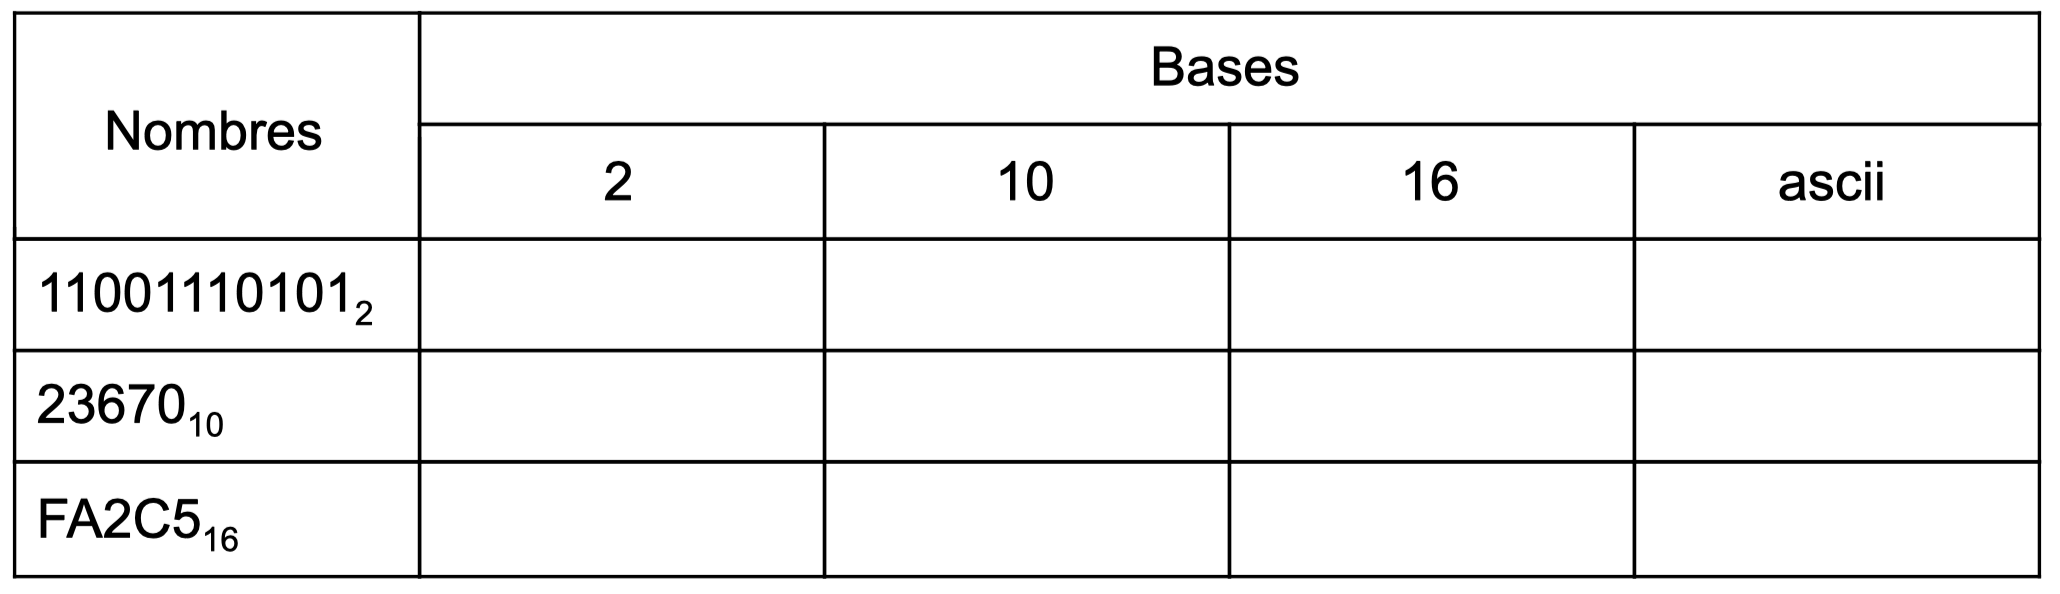
\includegraphics[scale=.27]{images/tableauconversion}
\end{figure}
\end{exercice}

\subsection{Annexe - Table ASCII étendue}
%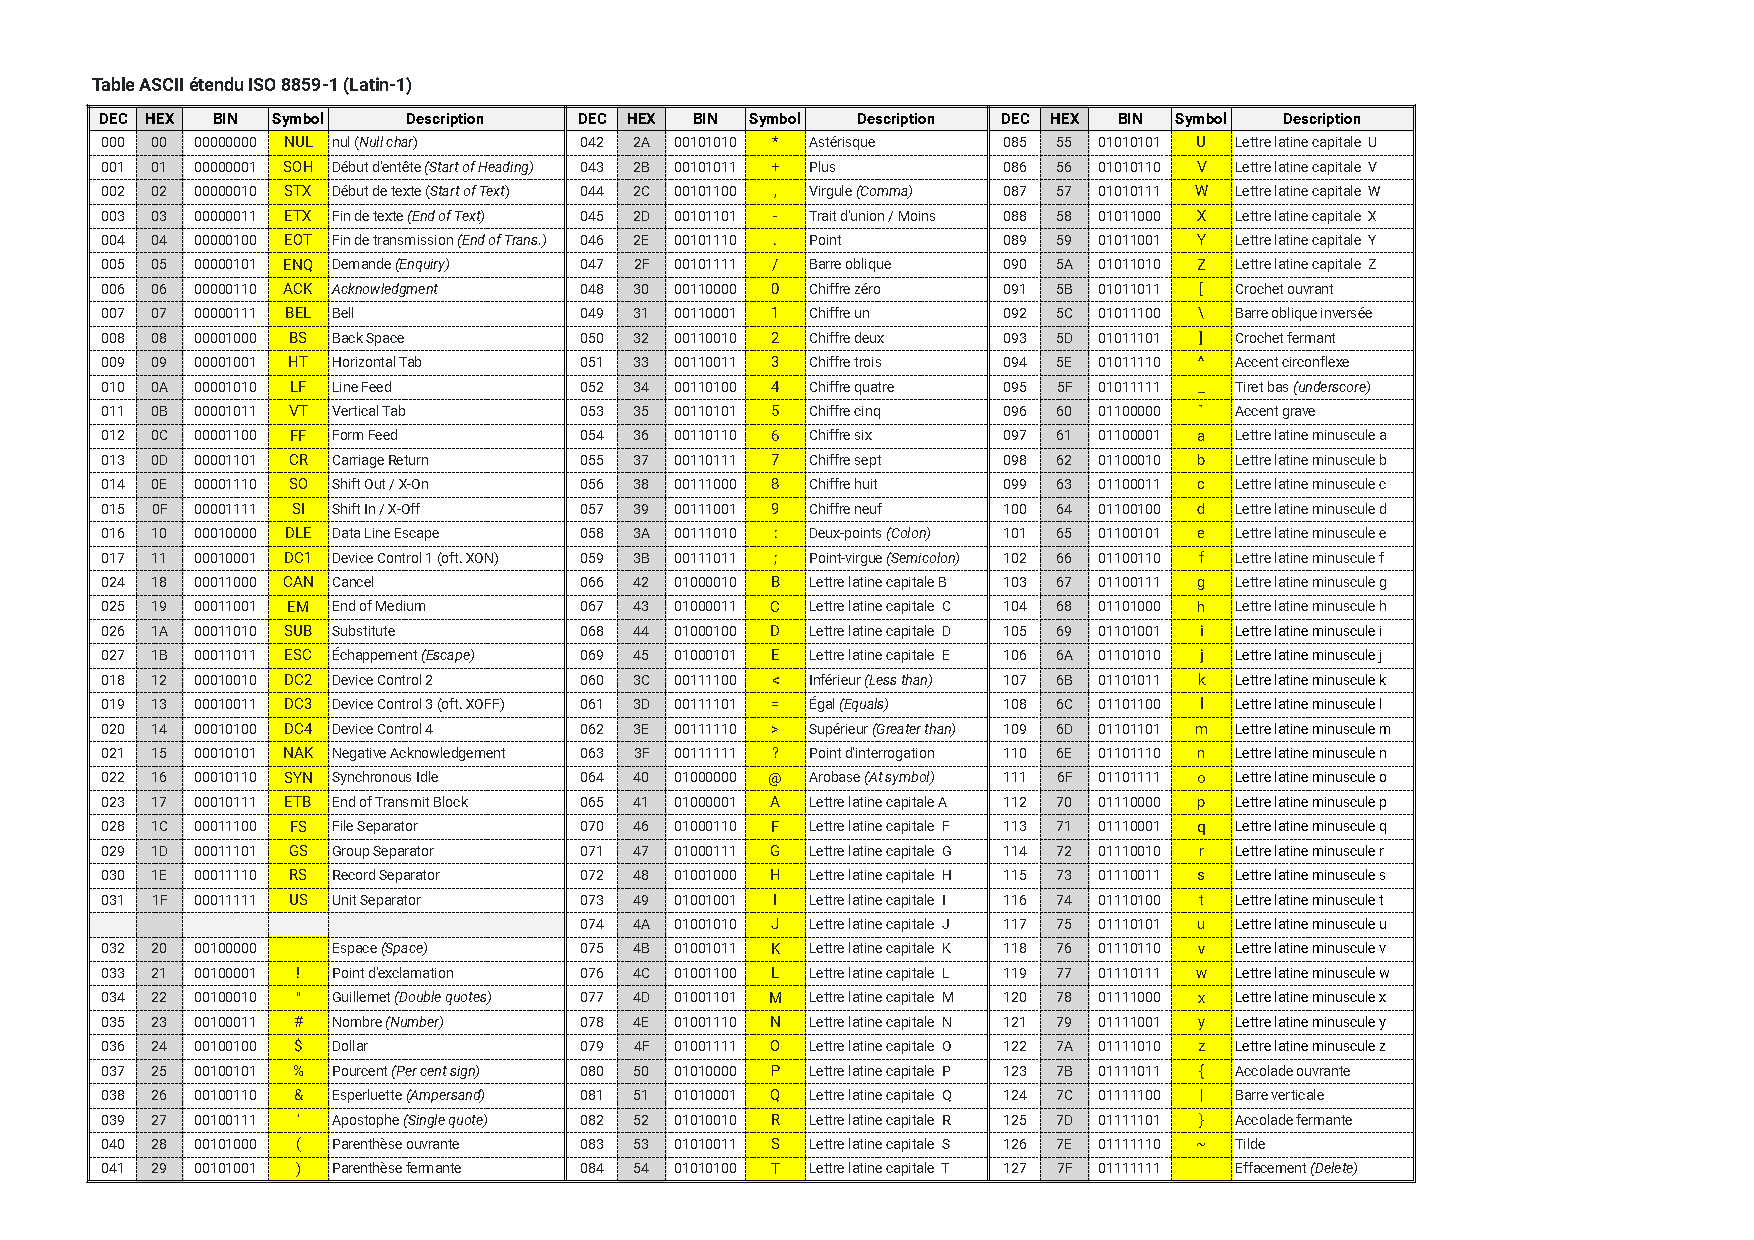
\includepdf[pages=-, angle=90]{images/3_Table-ASCII_étendue_MS.pdf}
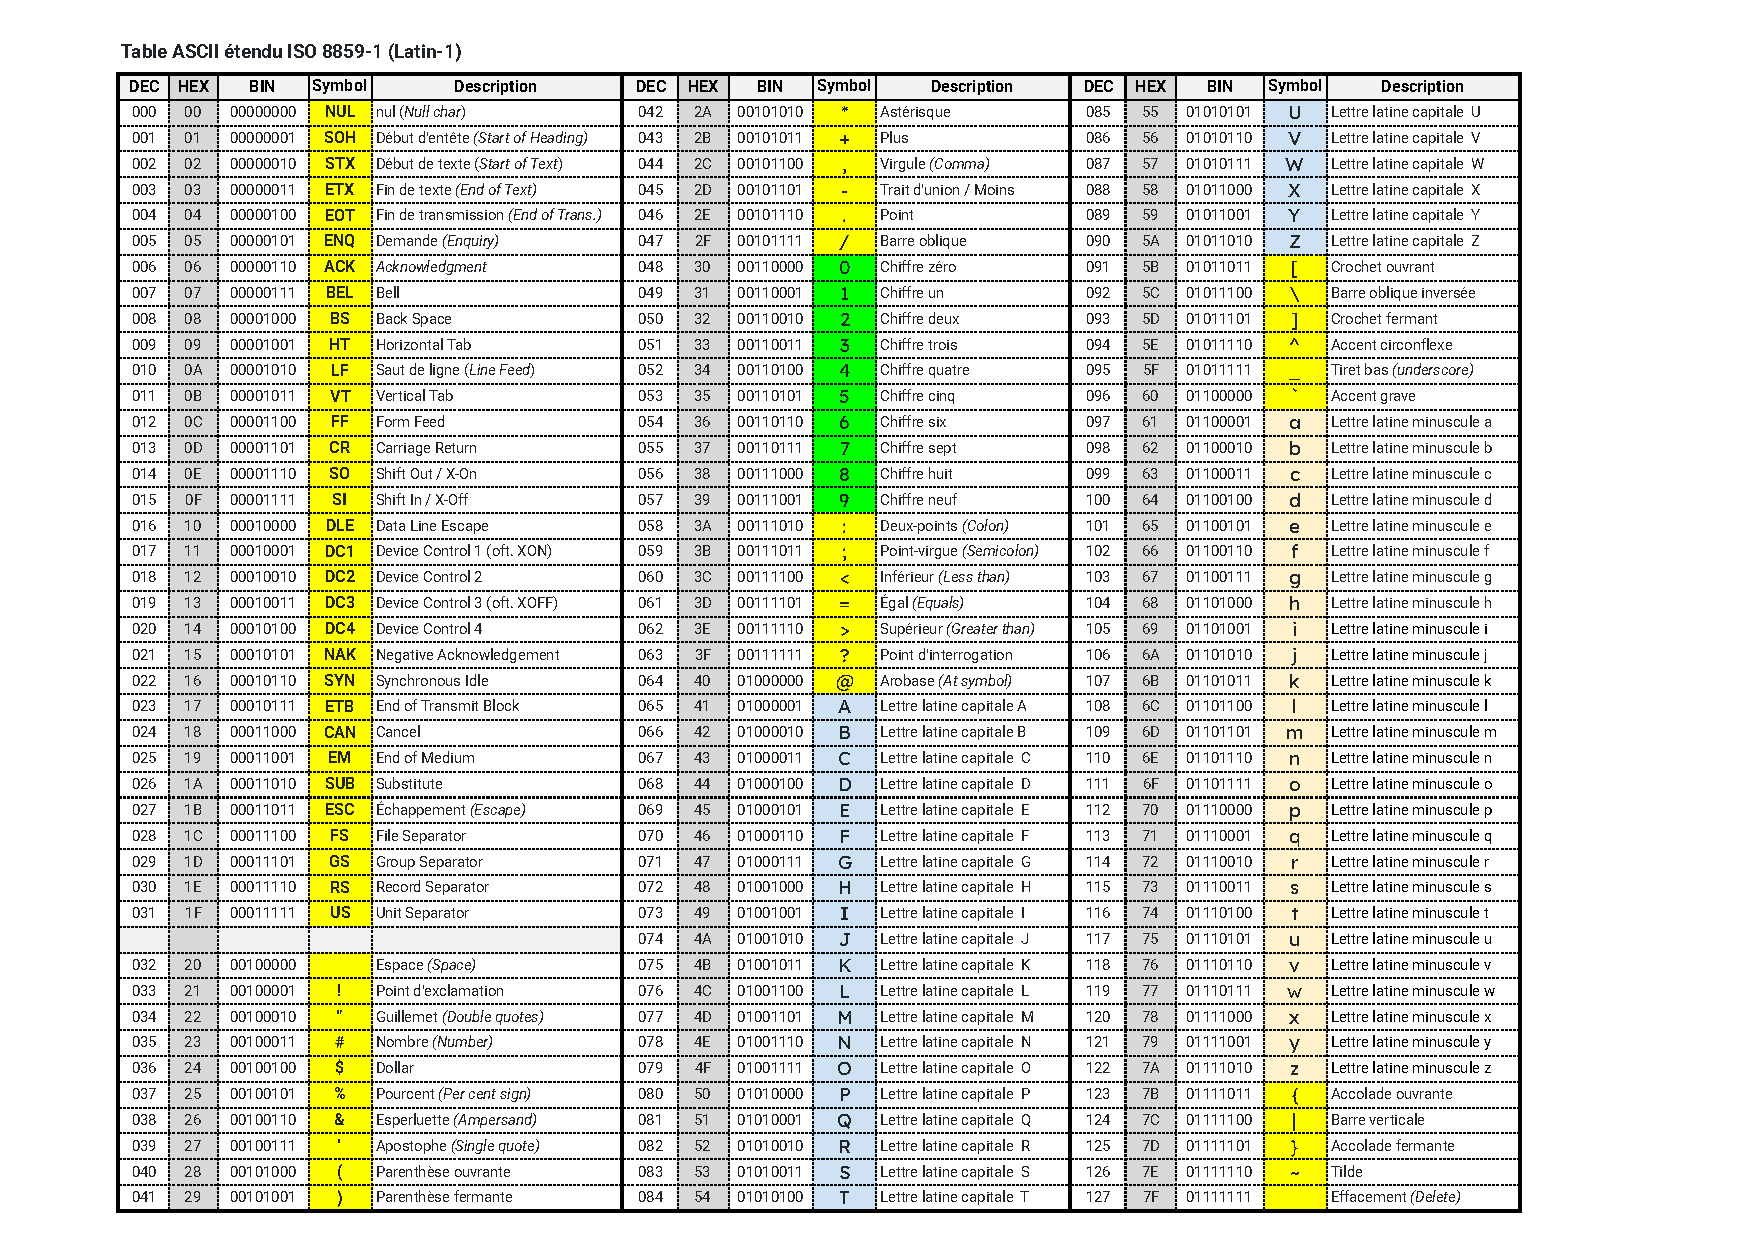
\includepdf[pages=-, angle=90]{images/03-Table-ASCII_étendue_FR.pdf}
\end{document}
